% 结构风格候选，使用支持中文的LaTeX文档。
\begin{figure*}[t]
\centering
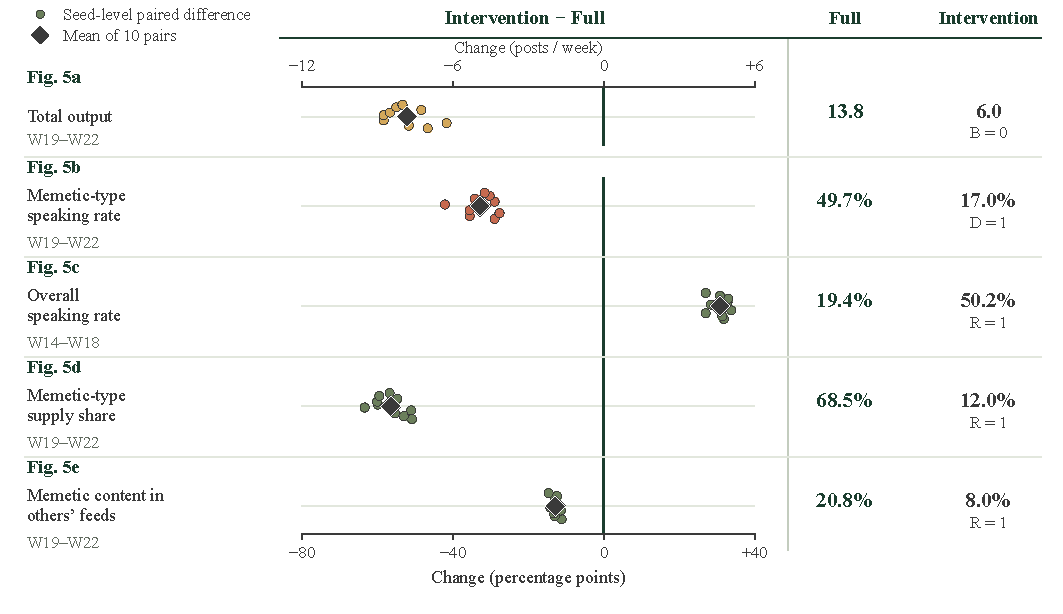
\includegraphics[width=\textwidth]{figure_05_effect_table_v1.pdf}
\caption{表达组件干预对参与、供给与可见位置的配对变化。（a）B=0条件下W19—W22的平均每周总供给；（b）D=1条件下同期玩梗型作者的发言率；（c）R=1条件下W14—W18全体作者的发言率；（d）、（e）分别为R=1条件下W19—W22玩梗型作者的供给份额及其他作者信息流中的玩梗内容比例。彩色圆点为同一种子内“干预−完整模型”的差值，黑色菱形为10个配对差值的均值，竖线表示零变化。图5a的差值单位为帖/周，图5b—e为百分点；右侧两列保留完整模型与干预条件的原单位均值。各项比较均在兴趣策展制度下进行，每条件包含10个种子，完整模型复用对应主实验，人口构成、外部输入与行动安排保持一致。图5e计入外部帖和生成帖，以其他作者实际获得的信息流展示为分母。}
\label{fig:figure_05_effect_table_v1}
\end{figure*}
